\section{TRISO Fuel}
\label{sec:triso_fuel}

In this work, we adapt the approach of Bachmann et al.
\cite{bachmann_enrichment_2021} to focus on \gls{triso} fueled reactor designs
alongside traditional fuel forms at various enrichments. \gls{triso} is not a
classification of enrichment; several reactor designs use different fuel
enrichments that are all \gls{triso}. Here we will distinguish the
production of \gls{triso} from the traditional metallic fuels used in
\glspl{lwr} outlined in Section \ref{sec:nfc}.

Coating the fuel particles is a critical step in the fabrication of \gls{triso}
fuel, and the idea has existed in nuclear fuel design spaces since the 1950s
\cite{price_dragon_2012} with the Dragon project. In 1957, the Harwell facility
began coating spherical fuel particles, and in 1961, researchers modified the
particle coating to include a silicon carbide layer to trap cesium, strontium,
and barium--which diffused through the single pyrolytic carbon layer.
Concurrently, in 1958, a report to the \gls{aec} introduced the concept of a
pebble bed pile (first proposed by Daniels
\cite{f_b_daniels_suggestions_1944}) to the broader nuclear community.
Researchers in Germany, China, and the UK have proposed, built, and operated
similar designs since then, with companies in the \gls{usa} looking to deploy
modern versions of the technology.

In a 2019 paper, authors Demkowicz, Liu, and Hunn \cite{particle_review_2019}
authors describe the fuel as a particle encapsulated in layers of pyrolytic
carbon and silicon carbide; a \gls{fbcvd} applies each of these layers. As
shown in Figure \ref{fig:triso_layers}, the layers are frequently ordered with
a fuel kernel at the center, followed by layers of porous carbon buffer, inner
pyrolytic carbon, silicon carbide, and outer pyrolytic carbon. The fuel kernel
is typically composed of uranium dioxide, and it is surrounded by a porous
carbon buffer using acetylene in the \gls{fbcvd} as it has a relatively low
density. The silicon carbide layer encapsulates the pyrolytic carbon layers and
provides a barrier to fission products. A mix of methyltrichlorosilane and
hydrogen is sufficient for SiC deposition without argon. The inner and outer
pyrolytic carbon layers isolate the silicon carbide layer and provide a barrier
to the coolant; the \gls{fbcvd} applies these layers using a mix of propylene,
acetylene, and argon.

\begin{figure}[H]
    \centering
    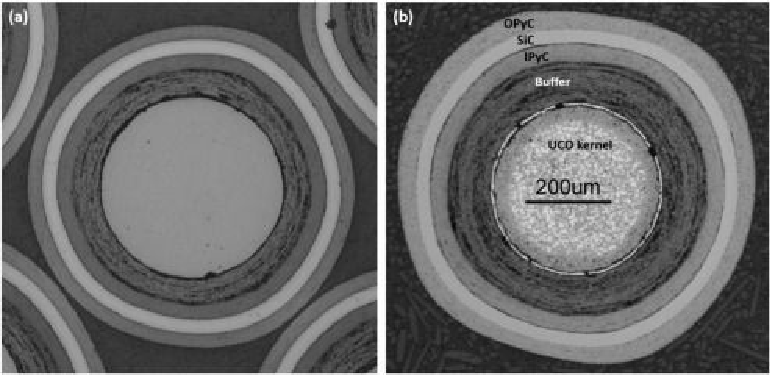
\includegraphics[scale=0.98]{images/triso_review/triso_layers.pdf}
    \caption{TRISO Fuel Particle Layers \cite{particle_review_2019}}
    \label{fig:triso_layers}
\end{figure}

Through a heat and pressure setting process, fabricators create a fuel matrix
that accepts the coated particles. These matrices hold the \gls{triso}
particles in graphite and carbonized resin and are set under heat and pressure,
often overcoated to prevent particle-particle interactions. The resulting fuel
type is incredibly robust and can reduce proliferation concerns due to the
difficulty separating the particles from the matrix and the fuel from the
particles. The fuel can withstand high temperatures and burnups, which can be
advantageous in reactor designs that require high temperatures for efficient
operation.